\documentclass[a4paper,oneside,14pt]{extreport}

\usepackage[T2A]{fontenc}
\usepackage[utf8]{inputenc}
\usepackage[english,russian]{babel}

\usepackage[left=30mm, right=10mm, top=20mm, bottom=20mm, bindingoffset=0cm]{geometry}

\usepackage{microtype}
\usepackage{tikz}

\usepackage{setspace}
\onehalfspacing
\usepackage{graphicx}
\usepackage{indentfirst}
\setlength{\parindent}{12.5mm}

\usepackage{titlesec}
\titleformat{\chapter}{\LARGE\bfseries}{\thechapter}{10pt}{\LARGE\bfseries}
\titlespacing*{\chapter}{0pt}{-20pt}{10pt}
\titleformat{\section}{\large\bfseries}{\thesection}{10pt}{\large\bfseries}
\titlespacing*{\section}{0pt}{0pt}{10pt}
\titleformat{\subsection}{\normalsize\bfseries}{\thesubsection}{10pt}{\normalsize\bfseries}
\titlespacing*{\subsection}{0pt}{5pt}{5pt}

\addto{\caption}{\renewcommand*{\contentsname}{Содержание}}
\usepackage[square,sort,comma,numbers]{natbib}
\renewcommand{\bibsection}{\chapter*{Список литературы}}

\usepackage{caption}

\usepackage{wrapfig}
\usepackage{float}
\usepackage{listings}
\usepackage{graphicx}
\graphicspath{{.}}
\newcommand{\imgwc}[4]
{
	\begin{figure}[#1]
		\center{\includegraphics[width=#2]{inc/img/#3}}
		\caption{#4}
		\label{img:#3}
	\end{figure}
}
\newcommand{\imghc}[4]
{
	\begin{figure}[#1]
		\center{\includegraphics[height=#2]{inc/img/#3}}
		\caption{#4}
		\label{img:#3}
	\end{figure}
}
\newcommand{\imgsc}[4]
{
	\begin{figure}[#1]
		\center{\includegraphics[scale=#2]{inc/img/#3}}
		\caption{#4}
		\label{img:#3}
	\end{figure}
}

\usepackage{pgfplots}
\pgfplotsset{compat=newest}

\usepackage{listings}
\usepackage{listingsutf8}
\lstset{
	basicstyle=\footnotesize\ttfamily,
	keywordstyle=\color{blue},
	stringstyle=\color{red},
	commentstyle=\color{gray},
	numbers=left,
	numberstyle=\tiny,
	numbersep=5pt,
	frame=false,
	breaklines=true,
	breakatwhitespace=true,
	inputencoding=utf8/koi8-r
}

\newcommand{\code}[1]{\texttt{#1}}

\usepackage{amsmath}
\usepackage{mathtools}
\usepackage{amssymb}

\usepackage[unicode]{hyperref}
\hypersetup{hidelinks}

\makeatletter
\newcommand{\vhrulefill}[1]
{
	\leavevmode\leaders\hrule\@height#1\hfill \kern\z@
}
\makeatother


\begin{document}
	\pagenumbering{Alph}
\documentclass[../report.tex]{subfiles}
\graphicspath{{\subfix{../images/}}}

\begin{document}
\thispagestyle{empty}
\doublespacing
\noindent
\begin{minipage}[l]{0.15\textwidth}
	\centering
	
\includegraphics{bmstu_low}
\end{minipage}
% нельзя делать пустую строку
\begin{minipage}[r]{0.85\textwidth}
	\centering\bfseries\singlespacing
	Министерство науки и высшего образования Российской Федерации\\
Федеральное государственное бюджетное образовательное учреждение\\
высшего образования\\
«Московский государственный технический университет\\
имени Н.Э. Баумана\\
(национальный исследовательский университет)»\\
(МГТУ им. Н.Э. Баумана)
\end{minipage}

\vspace*{5mm}
\noindent
\rule{\textwidth}{3pt}

\noindent
\MakeUppercase{Факультет}
\underline{«Информатика и системы управления»}

\noindent
\MakeUppercase{Кафедра}
\underline{«Программное обеспечение ЭВМ и информационные технологии»}

\vspace*{4cm}

\noindent
\center{
\textbf{
\MakeUppercase{Отчет\\
о лабораторной работе №5
}\\
\MakeUppercase{Конвеерная обработка данных}\\
по дисциплине:\\
«Анализ алгоритмов»
}}

\vspace*{3cm}

\begin{FlushLeft}
Руководитель: ст. преп. каф. ИУ7 \noindent\underline{\makebox[3em][l]{}} Волкова Л.Л.\\
Исполнитель: студ. гр. ИУ7-55Б \noindent\underline{\makebox[3em][l]{}} Муравьев И.А.
\end{FlushLeft}

\vspace*{\fill}
\center{
Москва 2021
}


\end{document}
\pagenumbering{arabic}
\newpage
\tableofcontents
\lstset{
	language = python,
	basicstyle=\small\sffamily,
	numbers=left,
	numberstyle=\tiny,
	stepnumber=1,
	numbersep=5pt,
	xleftmargin =.19in,
	showspaces=false,
	showstringspaces=false,
	showtabs=false,
	frame=single,
	tabsize=2,
	captionpos=t,
	breaklines=true,
	breakatwhitespace=false,
	escapeinside={\#*}{*)}
}

\newpage

\addcontentsline{toc}{chapter}{Введение}
\chapter*{Введение}
Конвейер — способ организации вычислений, используемый в современных процессорах и контроллерах с целью повышения их производительности (увеличения числа инструкций, выполняемых в единицу времени — эксплуатация параллелизма на уровне инструкций), технология, используемая при разработке компьютеров и других цифровых электронных устройств.

Сам термин <<конвейер>> пришёл из промышленности, где используется подобный принцип работы — материал автоматически подтягивается по ленте конвейера к рабочему, который осуществляет с ним необходимые действия, следующий за ним рабочий выполняет свои функции над получившейся заготовкой, следующий делает ещё что-то. Таким образом, к концу конвейера цепочка рабочих полностью выполняет все поставленные задачи, сохраняя высокий темп производства. Например, если на самую медленную операцию затрачивается одна минута, то каждая деталь будет сходить с конвейера через одну минуту. В процессорах роль рабочих исполняют функциональные модули, входящие в состав процессора.


\textbf{Целью данной работы} является реализация асинхронного взаимодействия потоков на примере конвейерной обработки данных.

Для достижения поставленной цели необходимо выполнить следующие \textbf{задачи:}
\begin{enumerate}
	\item Изучить асинхронное взаимодействие на примере конвейерной обработки данных.
	\item Привести схему конвейерных вычислений.
	\item Описать используемые структуры данных.
	\item Определить средства программной реализации.
	\item Реализовать и протестировать ПО.
	\item Провести сравнительный последовательной и конвейерной реализации по затрачиваемым ресурсам (времени работы).
	\item Изучить время, затрачиваемое на нахождение заявки в очереди к каждому этапу конвейера.
\end{enumerate}
\newpage

\chapter{Аналитическая часть}	
В данном разделе рассматриваются принципы и идея конвейерной обработки данных, а также приводится описание решаемой задачи и выделенных стадий конвейерной обработки.
	
\section{Описание конвейерной обработки данных}
Конвейер\cite{conveyor} — способ организации вычислений, используемый в современных процессорах и контроллерах с целью повышения их производительности (увеличения числа инструкций, выполняемых в единицу времени — эксплуатация параллелизма на уровне инструкций), технология, используемая при разработке компьютеров и других цифровых электронных устройств.

Идея заключается в параллельном выполнении нескольких инструкций процессора. Сложные инструкции процессора представляются в виде последовательности более простых стадий. Вместо выполнения инструкций последовательно (ожидания завершения конца одной инструкции и перехода к следующей), следующая инструкция может выполняться через несколько стадий выполнения первой инструкции. Это позволяет управляющим цепям процессора получать инструкции со скоростью самой медленной стадии обработки, однако при этом намного быстрее, чем при выполнении эксклюзивной полной обработки каждой инструкции от начала до конца.

Многие современные процессоры управляются тактовым генератором. Процессор внутри состоит из логических элементов и ячеек памяти — триггеров. Когда приходит сигнал от тактового генератора, триггеры приобретают своё новое значение, и «логике» требуется некоторое время для декодирования новых значений. Затем приходит следующий сигнал от тактового генератора, триггеры принимают новые значения, и так далее. Разбивая последовательности логических элементов на более короткие и помещая триггеры между этими короткими последовательностями, уменьшают время, необходимое логике для обработки сигналов. В этом случае длительность одного такта процессора может быть соответственно уменьшена.

\section{Выделенные стадии конвейерной обработки}
В данной работе в качестве алгоритма, реализованного для конвейеризации, используется шифрование паролей с сохранением в базу данных. Таким образом, было выделено три ленты конвейера:
\begin{enumerate}
	\item Модификация исходных данных выбранным способом для обеспечения невозможности расшифровки без информации об используемом методе.
	\item Двойное последовательное хеширование полученной строки для большей безопасности.
	\item Загрузка полученного значение в базу данных.
\end{enumerate}

\section{Требования к программному обеспечению}
На основе приведенного алгоритма можно выдвинуть требования к разрабатываемому ПО:
\begin{itemize}
%	\item входные данные - размер матрицы (целое число), её элементы (вещественные числа, по желанию пользователя, в противном случае - генерация произвольной матрицы заданного размера);
	\item выходные данные - время работы последовательного выполнения действий, время работы конвейера, минимальное, среднее, максимальное времена ожидания заявки в очереди каждой из конвейерных лент - вещественные числа;
	\item наличие обработки некорректного ввода.
\end{itemize}

\section{Вывод}
Был рассмотрен алгоритм нахождения определителя квадратной матрицы размера $n \times n$, он независимо вычисляет слагаемые
для нахождения итогового определителя, что дает возможность для реализации параллельного варианта алгоритма. Выдвинуты требования к разрабатываемому ПО: работа с квадратными матрицами произвольного размера (целое число) с возможностью ввода элементов вещественного типа пользователем или генерацией матрицы заданного размера, на выходе - вещественное число, соответствующее вычисленному определителю матрицы, обработка некорректного ввода.
\newpage

\chapter{Конструкторская часть}
Данный раздел содержит схемы конвейерной обработки данных, последовательного и конвейерного алгоритма.

\section{Схемы алгоритмов}
В данном пункте раздела представлены схемы реализуемых в работе алгоритмов.

На рисунке~\ref{img:count_det} представлена схема организации конвейерных вычислений на примере конвейера с тремя лентами.
\begin{figure}[H]
	\centering
	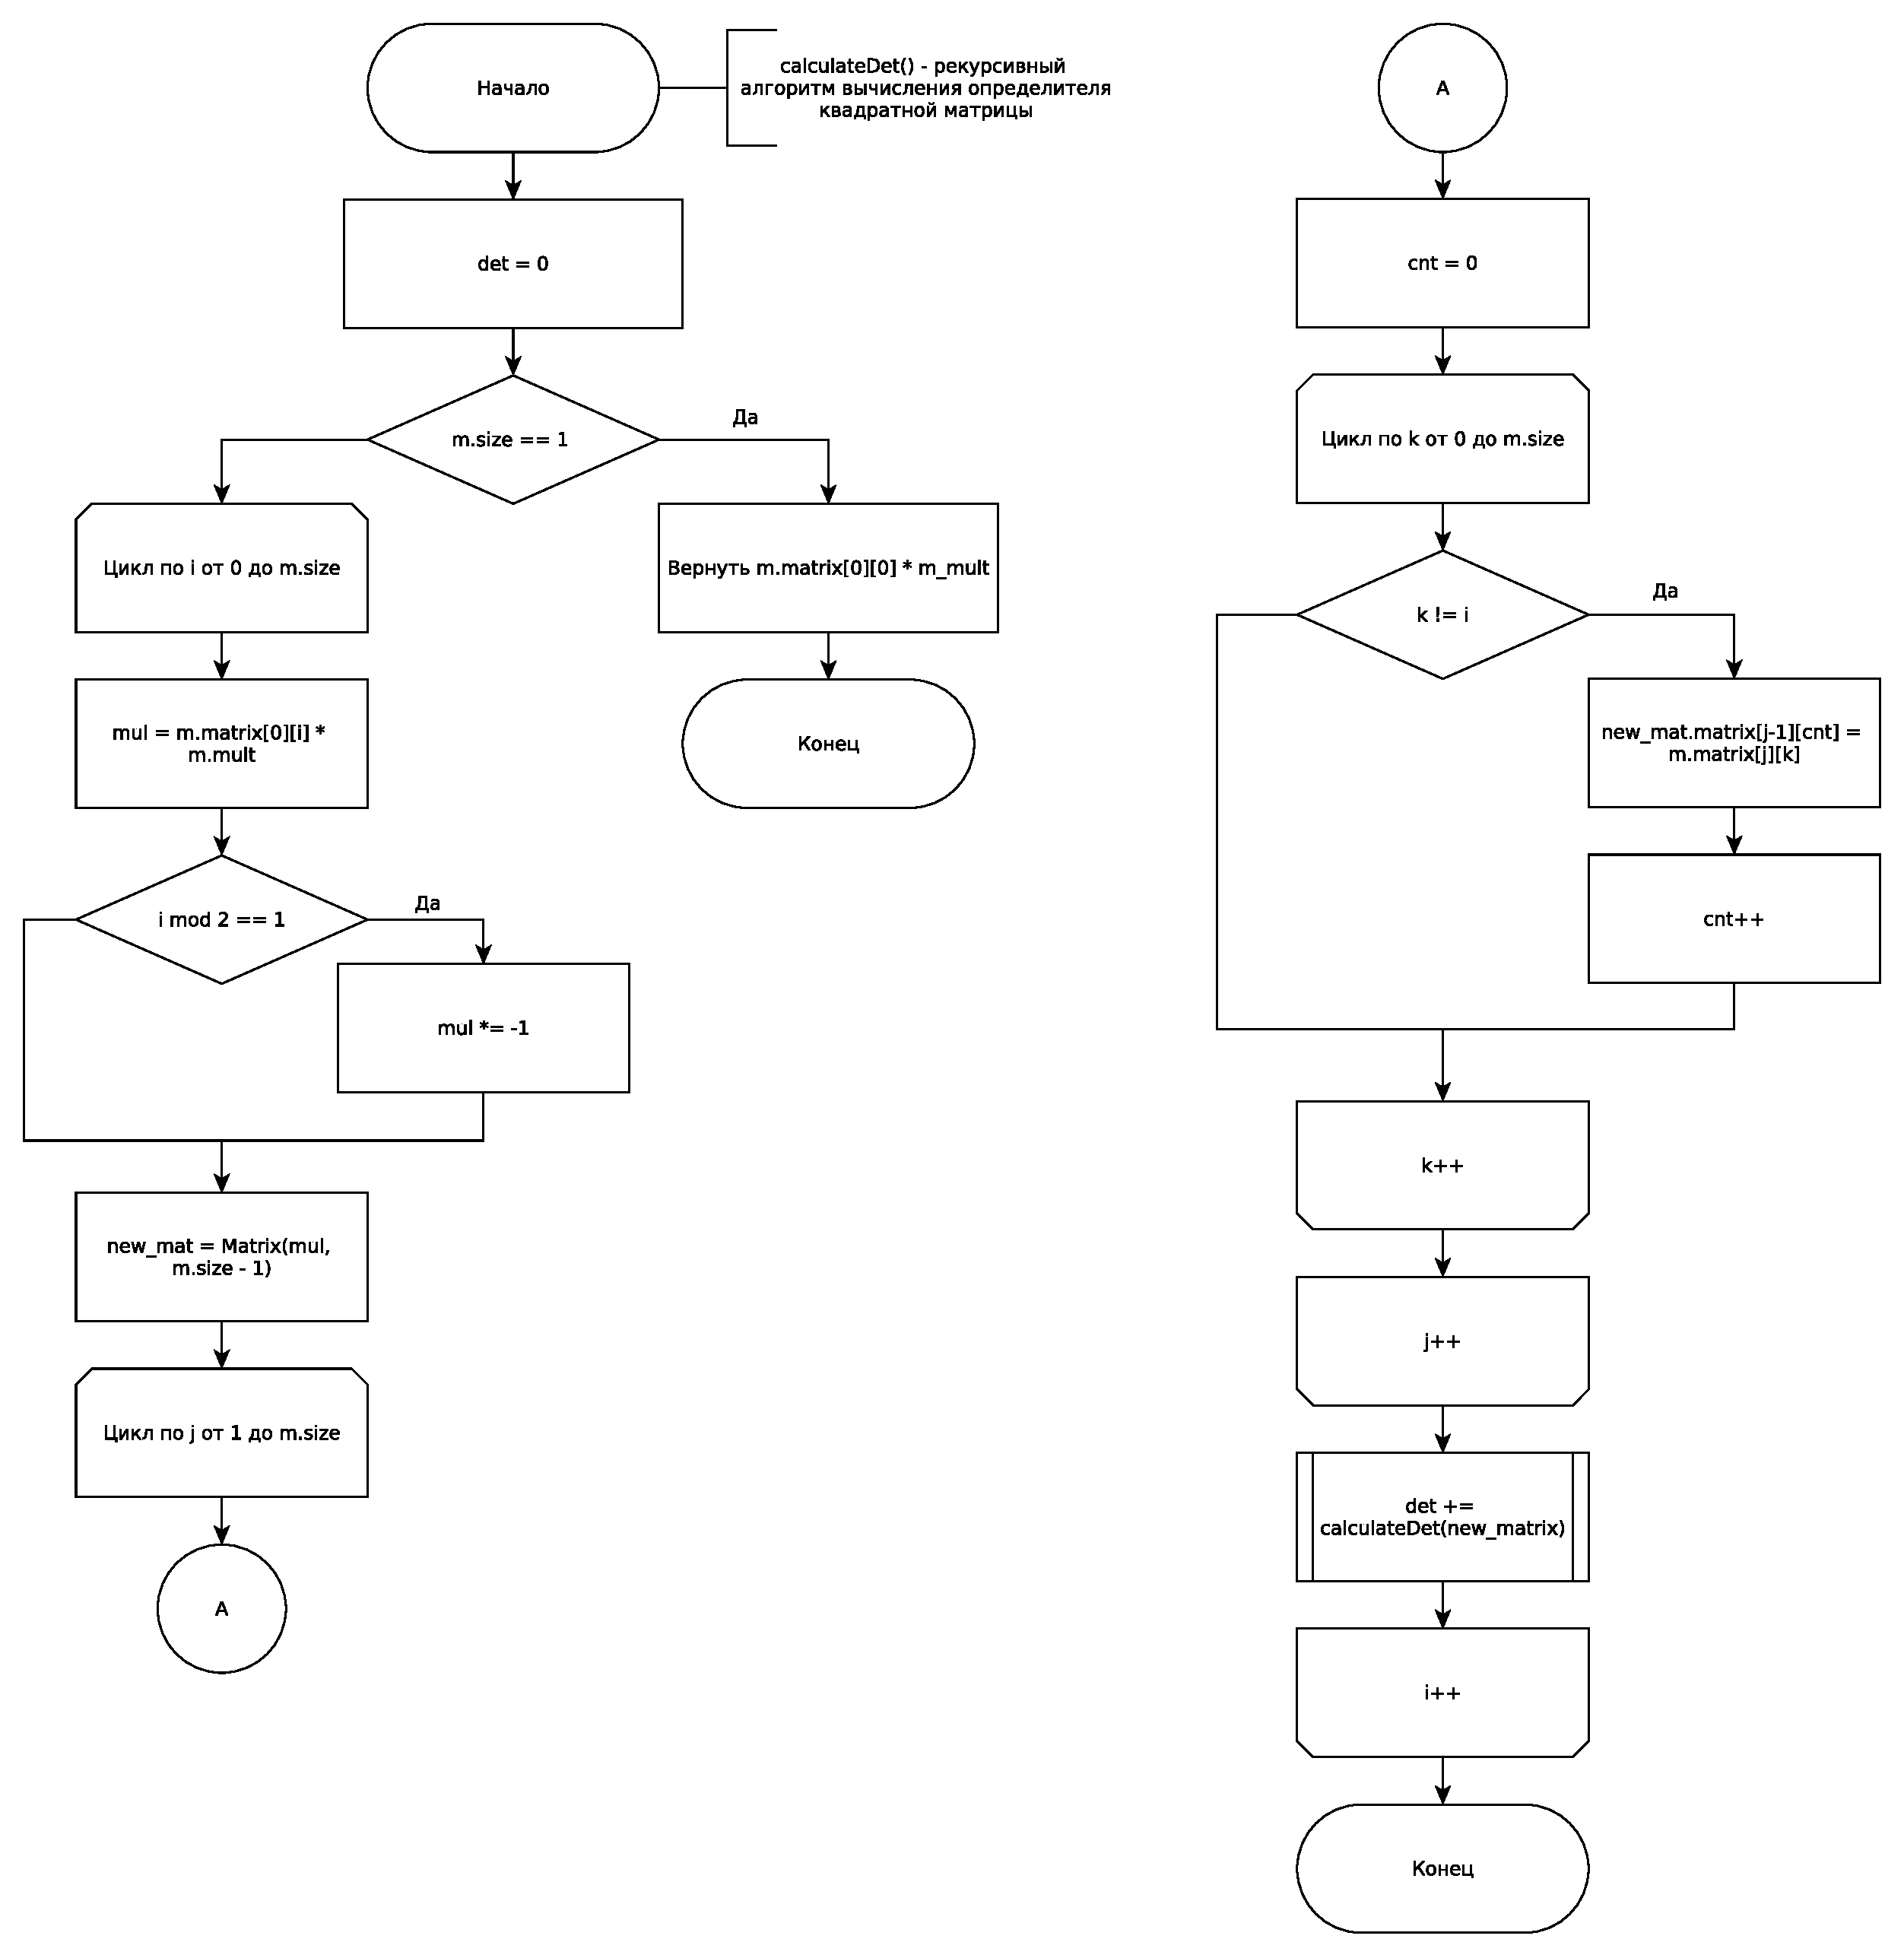
\includegraphics[width=1.00\linewidth]{images/count_det}
	\caption{Схема организации конвейера с тремя лентами}
	\label{img:count_det}
\end{figure}

На рисунке~\ref{img:thread_schema} представлена схема последовательного алгоритма шифрования и сохранения паролей.

\begin{figure}[H]
	\centering
	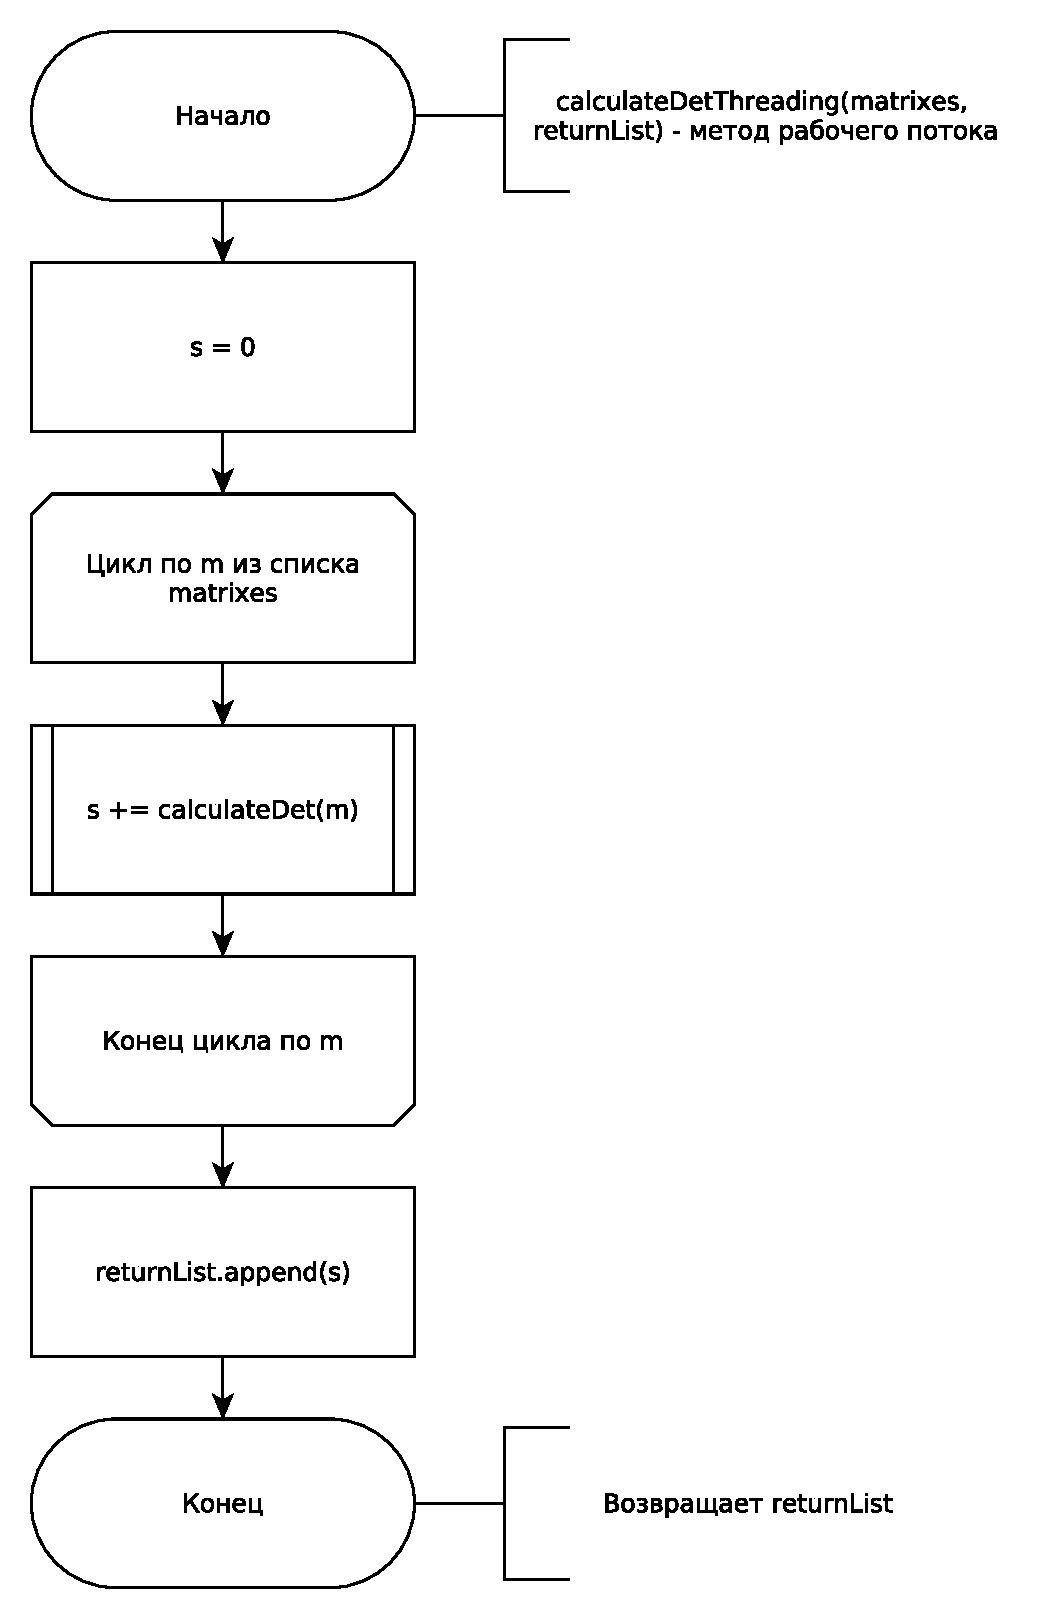
\includegraphics[width=0.85\linewidth]{images/thread_schema}
	\caption{Схема последовательного алгоритма}
	\label{img:thread_schema}
\end{figure}

На рисунках~\ref{img:solver_1} -~\ref{img:solver_2} представлена схема реализация алгоритма шифрования на конвейере с тремя лентами.

\begin{figure}[H]
	\centering
	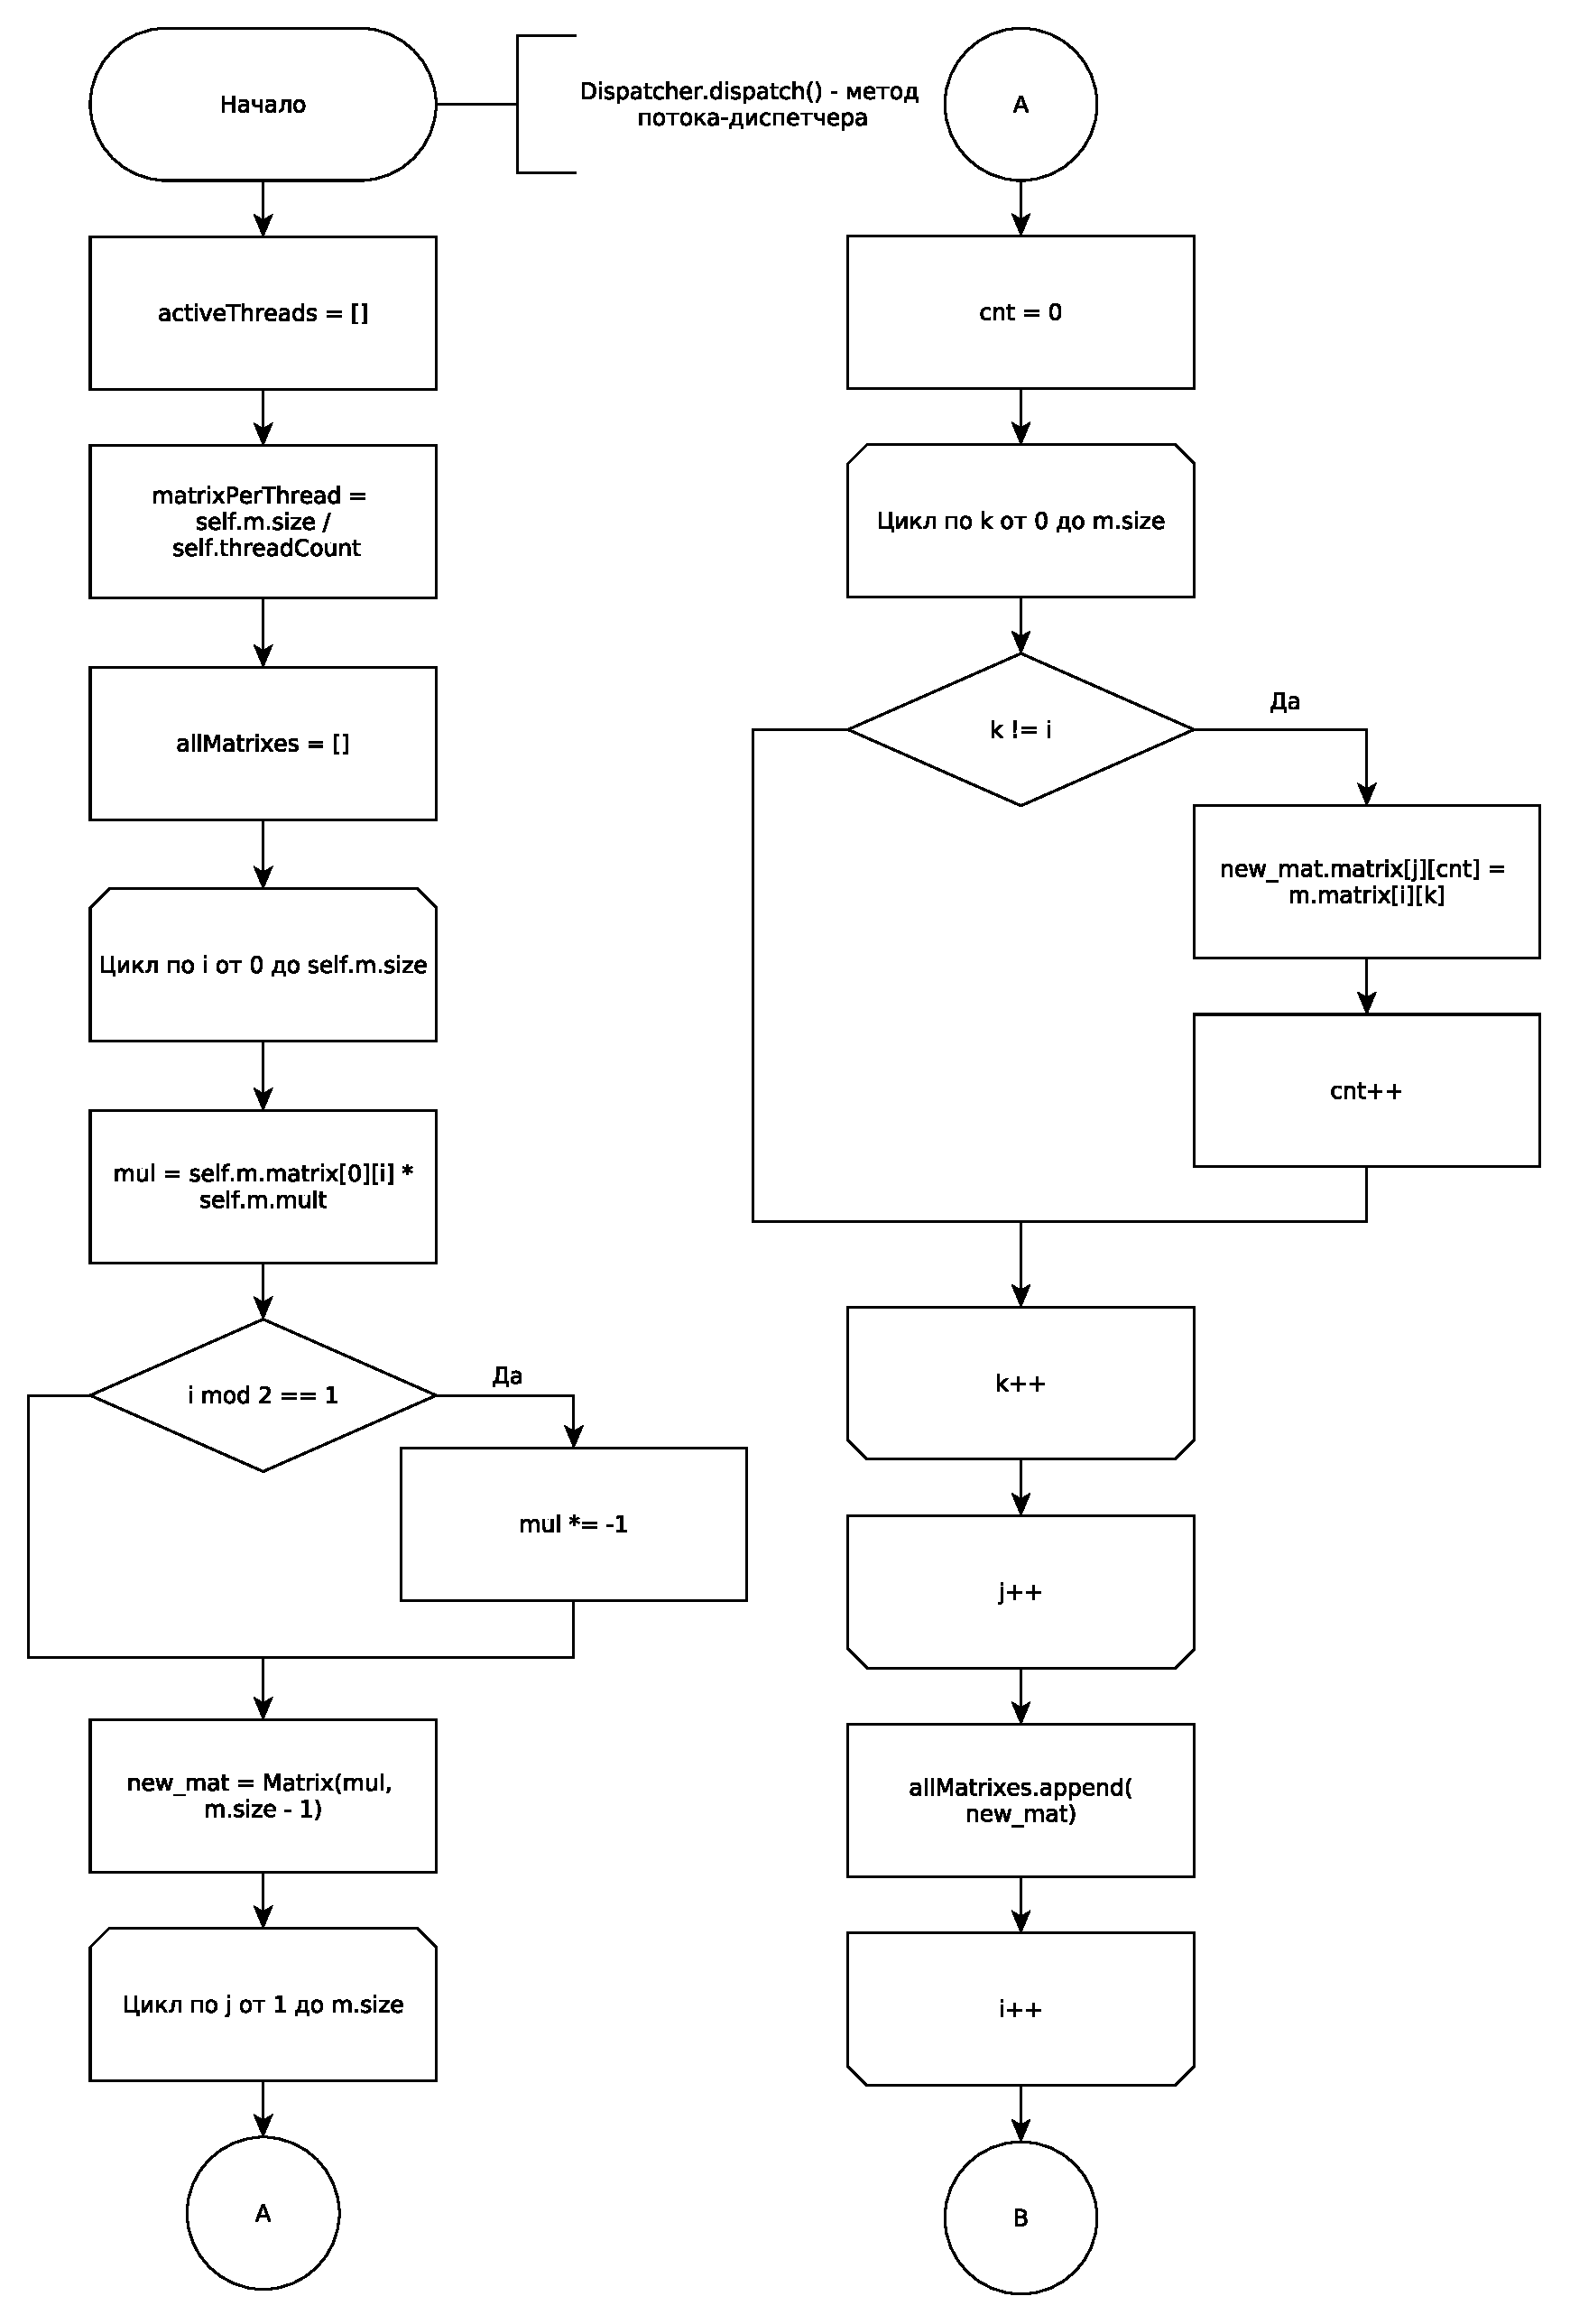
\includegraphics[width=0.85\linewidth]{images/solver_part_1}
	\caption{Схема алгоритма работы конвейерной обработки}
	\label{img:solver_1}
\end{figure}

\section{Структуры данных}
Для удобства работы были выделены следующие классы:
\begin{itemize}
	\item UserStats со следующими полями:
	\begin{itemize}
		\item login - строка, логин пользователя
	\end{itemize}
	\item mul - множитель минора (целое число, 1 для четных столбцов, -1 для нечетных с учетом начала нумерации с нуля);
	\item size - размер матрицы (целое число).
\end{itemize}

Для возможности генерации матриц, заполненных случайными элементами, класс Matrix содержит метод randomize.

Для управления потоками выделен класс Dispatcher со следующими полями:
\begin{itemize}
	\item m - матрица вещественных чисел, определитель которой необходимо вычислить;
	\item size - размер матрицы (целое число);
	\item threadCount - количество создаваемых потоков;
	\item returnList - список, разделяемый потоками, содержащий промежуточные вычисления определителей.
\end{itemize}

Таким образом, программа получает входные данные от пользователя (размер матрицы и её элементы), затем запускает вычисление определителя для разного количества потоков, чтобы сравнить время и корректность вычислений. Для деления на потоки исходная матрица, как и требуемое количество потоков, передается в конструктор класса Dispatcher и затем для каждого количества потоков вызывается метод dispatch, где происходит выделение "подматриц" потокам и запуск вычислительного процесса. Функция рабочего потока выполняет рекурсивное вычисление определителя для каждой переданной ему матрицы после чего вычисленное значение помещает в общий список, сумма которого вычисляется в главном потоке по завершении работы всех дочерних и возвращается как итоговый результат.

\section{Классы эквивалентности}
Для осуществления функционального тестирования ПО были выделены следующие классы эквивалентности:
\begin{itemize}
	\item матрица, состоящая из одного элемента;
	\item нулевая матрица;
	\item единичная матрица;
	\item произвольная матрица, определитель которой равен нулю;
	\item произвольная матрица, определитель которой не равен нулю.
\end{itemize}

\section{Вывод}
В данном разделе на основе приведенных в аналитическом разделе теоретических данных были составлены схемы алгоритмов для реализации в технологической части, в том числе, разделение вычисления определителя на потоки, выделены структуры данных и классы эквивалентности для дальнейшего тестирования программного обеспечения. 

\chapter{Технологическая часть}
Данный раздел содержит обоснование выбора языка и среды разработки, реализацию алгоритмов.

\section{Средства реализации}
Для реализации программы был выбран язык программирования Python~\cite{python}. Такой выбор обусловлен следующими причинами:
\begin{itemize}
	\item имеется большой опыт разработки;
	\item имеет большое количество расширений и библиотек, в том числе библиотеку для работы с потоками, измерения времени, построения графиков;
	\item обладает информативной документацией;
\end{itemize}

\section{Реализация алгоритмов}
В листингах \ref{lst:det_rec} - \ref{lst:work_thread} представлены реализации рассматриваемых алгоритмов.
%\newpage
\captionsetup{singlelinecheck=false, justification=raggedright}
\begin{lstlisting}[caption=Рекурсивный алгоритм вычисления определителя матрицы, label={lst:det_rec}]
def calculateDet(m: Matrix):
	s = 0                                                   
	if m.size == 1:                                         
		s = m.matrix[0][0] * m.mult                         
	else:                                                   
		for i in range(m.size):                             
			mul = m.matrix[0][i] * m.mult
			if i % 2 == 1:               
				mul *= -1                    
			size = m.size - 1            
			new_mat = Matrix(size, mul)  
			for j in range(1, m.size):   
				cnt = 0                      
				for k in range(m.size):      
					if k != i:                   
						new_mat.matrix[j - 1][cnt] = m.matrix[j][k] 
						cnt += 1                                    
			s += calculateDet(new_mat)                  
	return s      
\end{lstlisting}

\begin{lstlisting}[caption=Поток-диспетчер (часть 1)]
class Dispatcher:
	def __init__(self, size: int = 0, matrix: Matrix = None):
		self.m = matrix
		if size == 0: 
			size = 9
		if self.m is None:
			self.m = Matrix(size).randomize()
		self.threadCount = 1
		self.threadManager = Manager()
		self.returnList = self.threadManager.list()
	
	def dispatch(self):
		activeThreads = []
		matrixPerThread = self.m.size / self.threadCount
		allMatrixes = []
		for i in range(self.m.size):
			mul = self.m.matrix[0][i] * self.m.mult
			if i % 2 == 1:
				mul *= -1
			size = self.m.size - 1
			matrix = []
			for j in range(1, self.m.size):
				matrix.append([])
				for k in range(self.m.size):
					if k != i:
						matrix[-1].append(self.m.matrix[j][k])
			allMatrixes.append(Matrix(size, mul, matrix))
		startIndex = 0
		threadTasksCount = []
		for i in range(self.threadCount):
			endIndex = round(matrixPerThread * (i + 1))
			if i == self.threadCount - 1:  # last thread
				threadMatrixes = allMatrixes[startIndex:]
			else:
				threadMatrixes = allMatrixes[startIndex:endIndex]
			startIndex = endIndex
			activeThreads.append(
			Process(target=calculateDetThreading, args=(threadMatrixes, self.returnList)))
			threadTasksCount.append(len(threadMatrixes))
\end{lstlisting}
\begin{lstlisting}[caption=Поток-диспетчер (часть 2)]
		for thread in activeThreads:
			thread.start()
		for thread in activeThreads:
			thread.join()
		result = sum(self.returnList)
		self.returnList = self.threadManager.list()
		return result
\end{lstlisting}
%\newpage
\begin{lstlisting}[caption=Рабочий поток, label={lst:work_thread}]
def calculateDetThreading(matrixes, returnList: list):
	s = 0
	for m in matrixes:
		s += calculateDet(m)
	returnList.append(s)
\end{lstlisting}

\section{Тестирование}
В таблице \ref{tab:tests} представлены использованные для тестирования методом "черного ящика" данные, были рассмотрены все возможные тестовые случаи. Все тесты пройдены успешно.

\begin{table}[H]
	\begin{center}
		\captionsetup{justification=raggedleft, singlelinecheck=false}
		\caption[]{\label{tab:tests} Проведенные тесты}

	\begin{tabular}{|c|c|}
		\hline
		\rule[-1ex]{0pt}{2.5ex} Матрица & Определитель \\
		\hline
		\rule[-1ex]{0pt}{2.5ex} $\begin{pmatrix}
		9
		\end{pmatrix}$ & 9
		\\
		\hline
		\rule[-1ex]{0pt}{2.5ex} $\begin{pmatrix}
			0 & 0 \\
			0 & 0
		\end{pmatrix}$ & 0
		\\
		\hline
		\rule[-1ex]{0pt}{2.5ex} $\begin{pmatrix}
			1 & 0 & 0 \\
			0 & 1 & 0 \\
			0 & 0 & 1
		\end{pmatrix}$ & 1
		 \\
		\hline
		\rule[-1ex]{0pt}{2.5ex}	$\begin{pmatrix}
			1 & 2 & 3 \\
			4 & 5 & 6 \\
			7 & 8 & 12
		\end{pmatrix}$ & -9
		\\
		\hline
		\rule[-1ex]{0pt}{2.5ex} $\begin{pmatrix}
			1 & 2 & 3 & 4 \\
			5 & 6 & 7 & 8 \\
			9 & 10 & 11 & 12 \\
			13 & 14 & 15 & 16
		\end{pmatrix}$ & 0
		 \\
		 \hline
	\end{tabular}
\end{center}
\end{table}
\section{Выводы}
В данном разделе были реализованы и протестированы алгоритмы рекурсивного вычисления определителя и вычисления определителя с использованием многопоточности.
\newpage

\chapter{Экспериментальная часть}
В данном разделе сравниваются реализованные алгоритмы, дается сравнительная оценка затрат на время.

\section{Пример работы программы}
Пример работы программы представлен на рисунках \ref{fig:input_mat_ex} - \ref{fig:gener_ex}.
\captionsetup{singlelinecheck=true}
\begin{figure}[H]
	\centering
	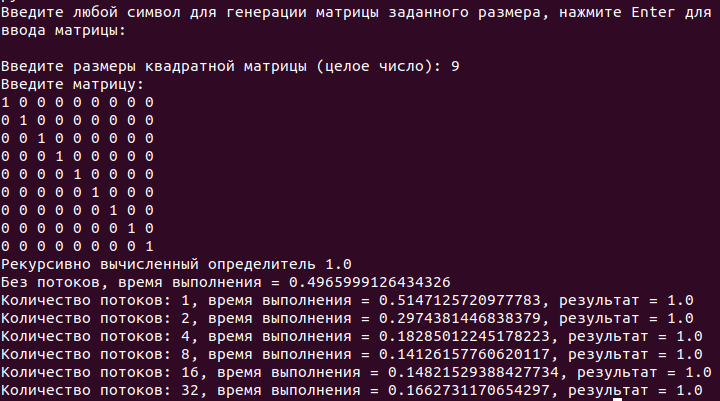
\includegraphics[width=1\linewidth]{images/input_mat_ex}
	\caption{Пример работы программы для вводимой матрицы}
	\label{fig:input_mat_ex}
\end{figure}

\begin{figure}[H]
	\centering
	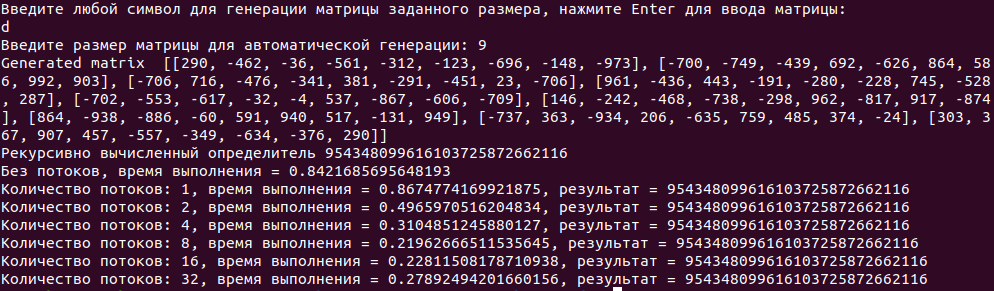
\includegraphics[width=1\linewidth]{images/generate_ex}
	\caption{Пример работы программы для вводимой матрицы}
	\label{fig:gener_ex}
\end{figure}


\section{Технические характеристики}
Технические характеристики устройства, на котором выполнялось исследование:
\begin{itemize}
	\item операционная система: Ubuntu 20.01 Linux x86\_64~\cite{ubuntu};
	\item оперативная память: 8 Гб;
	\item процессор: AMD Ryzen5 4500U~\cite{processor}:
	\begin{itemize}
		\item количество физических ядер: 6;
		\item количество логических ядер: 6.
	\end{itemize}
\end{itemize}

\section{Время выполнения алгоритмов}
Время выполнения алгоритмов измерялось на автоматически генерируемых квадратных матрицах необходимого размера (элементы которых - вещественные числа в диапазоне [-1000, 1000]) с использованием функции time библиотеки time. Усредненные результаты 10 замеров реального времени работы приведены в таблице ниже.

На рисунке \ref{fig:graph} представлена зависимость времени вычисления определителя матриц от размеров на основе таблицы \ref{tab:time}. Для матриц, размерность которых меньше 6, вычисление с использованием потоков занимает минимум в 1.3 раз (с увеличением коэффициента при увеличении количества потоков) больше времени в связи с превышением затратами на создание потоков затрат на последовательное вычисление определителя. Однако с увеличением размеров матрицы становится заметным преимущество использования параллельных вычислений. Таким образом, использование двух потоков дает выигрыш от 1.2 до 1.7 раз (для матриц, больших $6\times6$), четырех - от 1.2 до 2.8 раз (для матриц, больших $6\times6$), восьми - от 1.6 до 3.5 раз (матрицы от $7\times7$), шестнадцати - от 2.7 до 4.4 раз, для двадцати четырех - от 2.3 до 4.28 раз (матрицы от $8\times8$). Таким образом, с увеличением размерности матрицы, выигрыш от использования потоков увеличивается, при этом набольшим приростом, несмотря на получение преимуществ для матриц больших, чем те, на которых начинает выигрывать использование двух потоков ($6\times6$), обладает использование шестнадцати потоков, причем с ростом размерности матрицы выигрыш увеличивается соразмерно количеству потоков. Исключением является использование 24 потоков, который уступает в эффективности 16-и потокам из-за увеличения затрат на содержание потоков и управления ими.
\begin{table}[H]
	\begin{center}
		\captionsetup{justification=raggedleft, singlelinecheck=false}
		\caption{\label{tab:time} Время вычисления определителя матриц разных размеров в миллисекундах}
		\begin{tabular}{|c c c c c c c|} 
			\hline
			Размер&1 поток&2 потока&4 потока&8 потоков&16 потоков&24 потока\\ [0.5ex]
			\hline
	   		   4 &   12 &   14 &   16 &   22 &   36 &   51
	   		\\ 
	   		\hline
	   		5 &   14 &   15 &   16 &   23 &   37 &   51
	   		\\ 
	   		\hline
	   		6 &   22 &   18 &   19 &   23 &   37 &   50
	   		\\ 
	   		\hline
	   		7 &   50 &   33 &   29 &   31 &   46 &   58
	   		\\ 
	   		\hline
	   		8 &  251 &  138 &   80 &   83 &   94 &  108
	   		\\ 
	   		\hline
	   		9 & 2102 & 1212 &  756 &  599 &  476 &  491
	   		\\ 
	   		\hline
		\end{tabular}
	\end{center}
\end{table}

\begin{figure}[H]
	\centering
	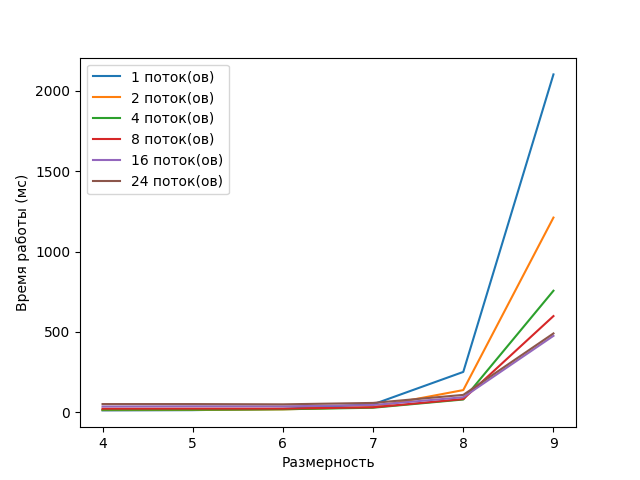
\includegraphics[width=0.9\linewidth]{images/graph}
	\caption{Зависимость времени работы алгоритмов от размера квадратной матрицы}
	\label{fig:graph}
\end{figure}

\section{Выводы}
В данном разделе были проведены измерения времени, затрачиваемого на вычисление определителя матрицы с использованием параллельных вычислений и без них.
На матрицах, размер которых не превышает 5, параллельные версии алгоритма оказались неэффективны. С увеличением размеров увеличивается эффективность использования параллельных вычислений, причем чем больше количество процессов, тем позже появляется выигрыш, но тем более существенным он оказывается. Исключением является использование 24 потоков в связи с большими затратами на обслуживание потоков в ядрах по сравнению с меньшим количеством потоков. Таким образом, выигрыш для 4 и 8 потоков проявляется на матрицах, больших $6\times6$ и составляет от 1.2 до 1.7 раз и от 1.2 до 2.8 раз соответственно, для восьми потоков - на матрицах, больших $7\times7$, от 1.5 до 3.5 раз, для 16 и 24 потоков - на матрицах, больших $8\times8$, от  2.7 до 4.4 раз и от 2.3 до 4.28 раз соответственно.
\newpage

\addcontentsline{toc}{chapter}{Заключение}
\chapter*{Заключение}
В процессе выполнения лабораторной работы были изучены и реализованы алгоритмы последовательного и параллельного вычисления определителя квадратной матрицы.

Было исследовано время выполнения выше обозначенных алгоритмов. В результате было выявлено, что на матрицах, размер которых не превышает 5, использование параллельных вычислений нецелесообразно из-за превышения затратами на содержание потоков затрат на последовательное вычисление определителя. С увеличением размеров увеличивается эффективность использования параллельных вычислений, причем чем больше количество процессов, тем позже появляется выигрыш, но тем более существенным он оказывается. Исключением является использование 24 потоков в связи с увеличением затрат на обслуживание потоков в ядрах по сравнению с 16 потоками. Таким образом, выигрыш для 4 и 8 потоков проявляется на матрицах, больших $6\times6$ и составляет от 1.2 до 1.7 раз и от 1.2 до 2.8 раз соответственно, для восьми потоков - на матрицах, больших $7\times7$, от 1.5 до 3.5 раз, для 16 и 24 потоков - на матрицах, больших $8\times8$, от  2.7 до 4.4 раз и от 2.3 до 4.28 раз соответственно. Наиболее эффективным для матриц, больших $8\times8$, является использование 16 потоков, для матриц $7\times7$ - 8 потоков, $6\times6$ - четырех.

\newpage
\addcontentsline{toc}{chapter}{Список литературы}

\bibliographystyle{utf8gost705u}
\bibliography{bib_lab_5}
\nocite{*}


\end{document}